\documentclass{beamer}
\usetheme{Juelich}

\title{Quantum Boltzmann Machines}
\subtitle{Applications in Quantitative Finance}
\author{Cameron Perot}
\institute{JSC}
\date{\today}
\titlegraphic{\includegraphics%
    [height=0.45\paperheight]{placeholder}
}

% packages
\usepackage{amssymb}
\usepackage{amsmath}
\usepackage{float}
\usepackage{graphicx}
\usepackage{braket}
\usepackage{multirow}
\usepackage{bbm}
\usepackage{mathtools}

\graphicspath{ {../../../artifacts/exact_analysis/}{../../../artifacts/plots/anneal_schedules/}{../../../results/plots/qbm/}{../../../results/plots/data_analysis/}{../../images/} }

% new commands
% Misc. commands
\newcommand{\CNOT}[2]{\text{C}_{#1}\text{NOT}_{#2}}
\newcommand{\SWAP}{\text{SWAP}}
\newcommand{\CZ}{\text{CZ}}
\newcommand{\tr}{\text{tr}}
\newcommand{\frt}{\frac{1}{\sqrt{2}}}
\newcommand{\Z}{\mathbb{Z}}
\newcommand{\R}{\mathbb{R}}
\newcommand{\N}{\mathbb{N}}
\newcommand{\mat}[1]{\mathbf{#1}}
\newcommand{\binset}{\{0,1\}}
\newcommand{\spause}{s_{\text{pause}}}
\newcommand{\tpause}{t_{\text{pause}}}
\newcommand{\Deltapause}{\Delta_{\text{pause}}}
\newcommand{\Deltaquench}{\Delta_{\text{quench}}}
\newcommand{\alphaquench}{\alpha_{\text{quench}}}
\renewcommand{\vec}[1]{\mathbf{#1}}
\newcommand{\basistwo}{\{\ket{00}, \ket{01}, \ket{10}, \ket{11}\}}
\DeclarePairedDelimiter{\norm}{\lVert}{\rVert}
\DeclarePairedDelimiter{\abs}{\lvert}{\rvert}

% Identity operator (on K^2)
\newcommand{\idtwo}{
    \begin{bmatrix}
        1 & 0 \\
        0 & 1
    \end{bmatrix}
}

% Hadamard operator
\newcommand{\Hgate}{
    \frac{1}{\sqrt{2}} \begin{bmatrix}
        1 & 1 \\
        1 & -1
    \end{bmatrix}
}

% T gate
\newcommand{\Tgate}{
    \begin{bmatrix}
        1 & 0 \\
        0 & e^{i \pi / 4}
    \end{bmatrix}
}

% T gate dag
\newcommand{\Tgatedag}{
    \begin{bmatrix}
        1 & 0 \\
        0 & e^{-i \pi / 4}
    \end{bmatrix}
}

% R_X
\newcommand{\RXGate}[1]{
    \begin{bmatrix}
        \cos\frac{#1}{2} & -i\sin\frac{#1}{2} \\
        -i\sin\frac{#1}{2} & \cos\frac{#1}{2}
    \end{bmatrix}
}

% R_Y
\newcommand{\RYGate}[1]{
    \begin{bmatrix}
        \cos\frac{#1}{2} & -\sin\frac{#1}{2} \\
        \sin\frac{#1}{2} & \cos\frac{#1}{2}
    \end{bmatrix}
}

% R_Z
\newcommand{\RZGate}[1]{
    \begin{bmatrix}
        e^{-i{#1}/2} & 0 \\
        0 & e^{i{#1}/2}
    \end{bmatrix}
}

% Pauli X operator
\newcommand{\XGate}{
    \begin{bmatrix}
        0 & 1 \\
        1 & 0
    \end{bmatrix}
}

% Pauli Y operator
\newcommand{\YGate}{
    \begin{bmatrix}
        0 & -i \\
        i & 0
    \end{bmatrix}
}

% Pauli Z operator
\newcommand{\ZGate}{
    \begin{bmatrix}
        1 & 0 \\
        0 & -1
    \end{bmatrix}
}

% The |0⟩ state in vector form
\newcommand{\zerostate}{
    \begin{bmatrix}
        1 \\
        0
    \end{bmatrix}
}

% The |1⟩ state in vector form
\newcommand{\onestate}{
    \begin{bmatrix}
        0 \\
        1
    \end{bmatrix}
}

% The |-⟩ state in vector form
\newcommand{\minusstatey}{
    \frac{1}{\sqrt{2}}
    \begin{bmatrix}
        1 \\
        -i
    \end{bmatrix}
}

% The |+⟩ state in vector form
\newcommand{\plusstatey}{
    \frac{1}{\sqrt{2}}
    \begin{bmatrix}
        1 \\
        i
    \end{bmatrix}
}

% The |-'⟩ state in vector form
\newcommand{\minusstate}{
    \frac{1}{\sqrt{2}}
    \begin{bmatrix}
        1 \\
        -1
    \end{bmatrix}
}

% The |+'⟩ state in vector form
\newcommand{\plusstate}{
    \frac{1}{\sqrt{2}}
    \begin{bmatrix}
        1 \\
        1
    \end{bmatrix}
}


\begin{document}
%----------------------------------------------------------------------------------------
% Title Page
%----------------------------------------------------------------------------------------

\maketitle

%----------------------------------------------------------------------------------------
% Table of Contents
%----------------------------------------------------------------------------------------

\begin{frame}
    \frametitle{Overview}
    \tableofcontents
\end{frame}

%----------------------------------------------------------------------------------------
% Quantum Boltzmann Machines
%----------------------------------------------------------------------------------------

\section{Quantum Boltzmann Machines}

\begin{frame}
    \frametitle{Quantum Boltzmann Machine (QBM)}
    QBM has the Hamiltonian given by
    \[
        H = -\sum_i \Gamma_i \sigma_i^x -\sum_i c_i \sigma_i^z - \sum_{i,j} w_{ij} \sigma_i^z \sigma_j^z
    \]
    with associated density operator
    \[
        \rho = \frac{1}{Z} e^{-H}
    \]
    where \( Z = \tr(e^{-H}) \) is the partition function.
\end{frame}

\begin{frame}
    \frametitle{QBM Optimization}
    The log-likelihood function is given by
    \[
        \ell = \sum_\vec{v} p_{\text{data}}(\vec{v}) \log\frac{\tr(\Lambda_\vec{v} e^{-H})}{\tr(e^{-H})}
    \]
    The log-likelihood is not efficient to optimize, rather it's best to maximize the lower bound (this is called a "bounded" QBM, or BQBM, or even a BQRBM when connectivity restrictions are imposed)
    \[
        \ell \ge \tilde{\ell} = \sum_\vec{v} p_{\text{data}}(\vec{v}) \log\frac{\tr(e^{-H_\vec{v}})}{\tr(e^{-H})}
    \]
    where \( H_\vec{v} = \braket{\vec{v} | H | \vec{v}} \) is the Hamiltonian "clamped" to the data vector \( \vec{v} \).
    This all leads to iterative updates of
    \begin{align*}
        \Delta c_i
            &= \eta (\overline{\braket{\sigma_i^z}_\vec{v}} - \braket{\sigma_i^z}) \\
        \Delta w_{ij}
            &= \eta (\overline{\braket{\sigma_i^z\sigma_j^z}_\vec{v}} - \braket{\sigma_i^z\sigma_j^z})
    \end{align*}
\end{frame}

\begin{frame}
    \frametitle{Mapping the QBM to the Annealer}
    The quantum annealer has Hamiltonian
    \[
        H(s) = -A(s) \sum_i \sigma_i^x + B(s) \bigg[ \sum_i h_i \sigma_i^z + \sum_{i,j} J_{ij} \sigma_i^z \sigma_j^z \bigg]
    \]
    In theory it should be possible to use the annealer to sample from this distribution if the evolution is frozen at some point \( s^* \) in the anneal process and the qubits are then read out. In practice this can be done by annealing slowly in the beginning up to some point, then annealing quickly to the end of the cycle (quenching)~\cite{amin_2018}.
    This allows us to translate our problem using
    \begin{align*}
        \Gamma_i
            &= \beta A(s^*) \\
        c_i
            &= -\beta B(s^*) h_i \\
        w_{ij}
            &= -\beta B(s^*) J_{ij}
    \end{align*}
\end{frame}

%----------------------------------------------------------------------------------------
% Anneal Schedule Analysis
%----------------------------------------------------------------------------------------

\section{Anneal Schedule Analysis}

\begin{frame}
    \frametitle{Anneal Schedules}
    Multiple different annealing schedules were tested.
    Namely, anneal schedules are in the form of \( (t, s) \) tuples
    \[
        [(0, 0), \ (\tpause, \spause), \ (\tpause + \Deltapause, \spause), \ (\tpause + \Deltapause + \Deltaquench, 1)]
    \]
    where \( \tpause = \spause \cdot t_a \).

    Chosen values were
    \begin{align*}
        t_a
            &\in \{20, 100\} \ [\mu\text{s}] \\
        \spause
            &\in \{0.25, 0.3, \dots, 0.7, 0.75\} \\
        \Deltapause
            &\in \{0, 10, 100, 1000\} \ [\mu\text{s}]
    \end{align*}
    The quench duration \( \Deltaquench \) was always chosen to be the fastest possible rate, which for the Advantage 5.1 system is defined by the maximum slope of \( \alphaquench = 2 \), i.e.
    \[
        \Deltaquench = \frac{1 - \spause}{\alphaquench}
    \]
\end{frame}

\begin{frame}
    \begin{figure}
        \includegraphics[width=0.65\linewidth]{t_pause=9.0,s_pause=0.45,pause_duration=10.0,quench_slope=2.0.png}
    \end{figure}
\end{frame}

\begin{frame}
    \frametitle{A Toy Problem}
    In essence we would like to match the samples we obtain from the annealer to a theoretical distribution, in particular that of the QBM.
    For this purpose, a small 12 qubit (BQRBM) problem was studied, with 8 visible units and 4 hidden units.
    Three different subproblems were studied with the weights and biases being normally distributed at different scales, i.e.,
    \begin{align*}
        h_i, J_{ij} &\sim \mathcal{N}(0, 0.01) \\
        h_i, J_{ij} &\sim \mathcal{N}(0, 0.1) \\
        h_i, J_{ij} &\sim \mathcal{N}(0, 1)
    \end{align*}
    For each set of weights and biases, the annealer was sampled the maximum number of times (sample sets with longer anneal schedules might have fewer samples as to satisfy the maximum QPU time constraint).
\end{frame}

\begin{frame}
    \frametitle{Sampling the Annealer}
    The D-Wave Advantage 5.1 system was sampled using \texttt{sample\_ising()} with the defined anneal schedule and auto scaling disabled.

    To generate more robust statistics, 10 random gauges were used in order to reduce any readout bias of the qubits.
    For a random vector \( \vec{r} \in \{-1,+1\}^{N} \) we can take
    \begin{align*}
        h_i &\rightarrow r_i h_i \\
        J_{ij} &\rightarrow r_i r_j J_{ij} \\
        (z_1, \dots, z_N) &\rightarrow (r_1 z_1, \dots, r_N z_N)
    \end{align*}
\end{frame}

\begin{frame}
    \frametitle{KL Divergence}
    The exact QBM distributions were computed and compared to the samples obtained from the annealer.
    A discrete approximation of the KL divergence was computed through the use of binning (32 bins) with smoothing, as a metric to help determine how much information is lost using the samples from the annealer to approximate the theoretical distribution.
    For each anneal schedule a heatmap of the KL divergence was generated for \( T = 0.001, 2, 4, \dots, 100 \) mK and \( s = 0, 0.01, \dots, 1 \), thus there is a lot of visual data to sort through.
\end{frame}

\begin{frame}
    \frametitle{\( h_i, J_{ij} \sim \mathcal{N}(0, 0.01) \)}
    \begin{figure}
        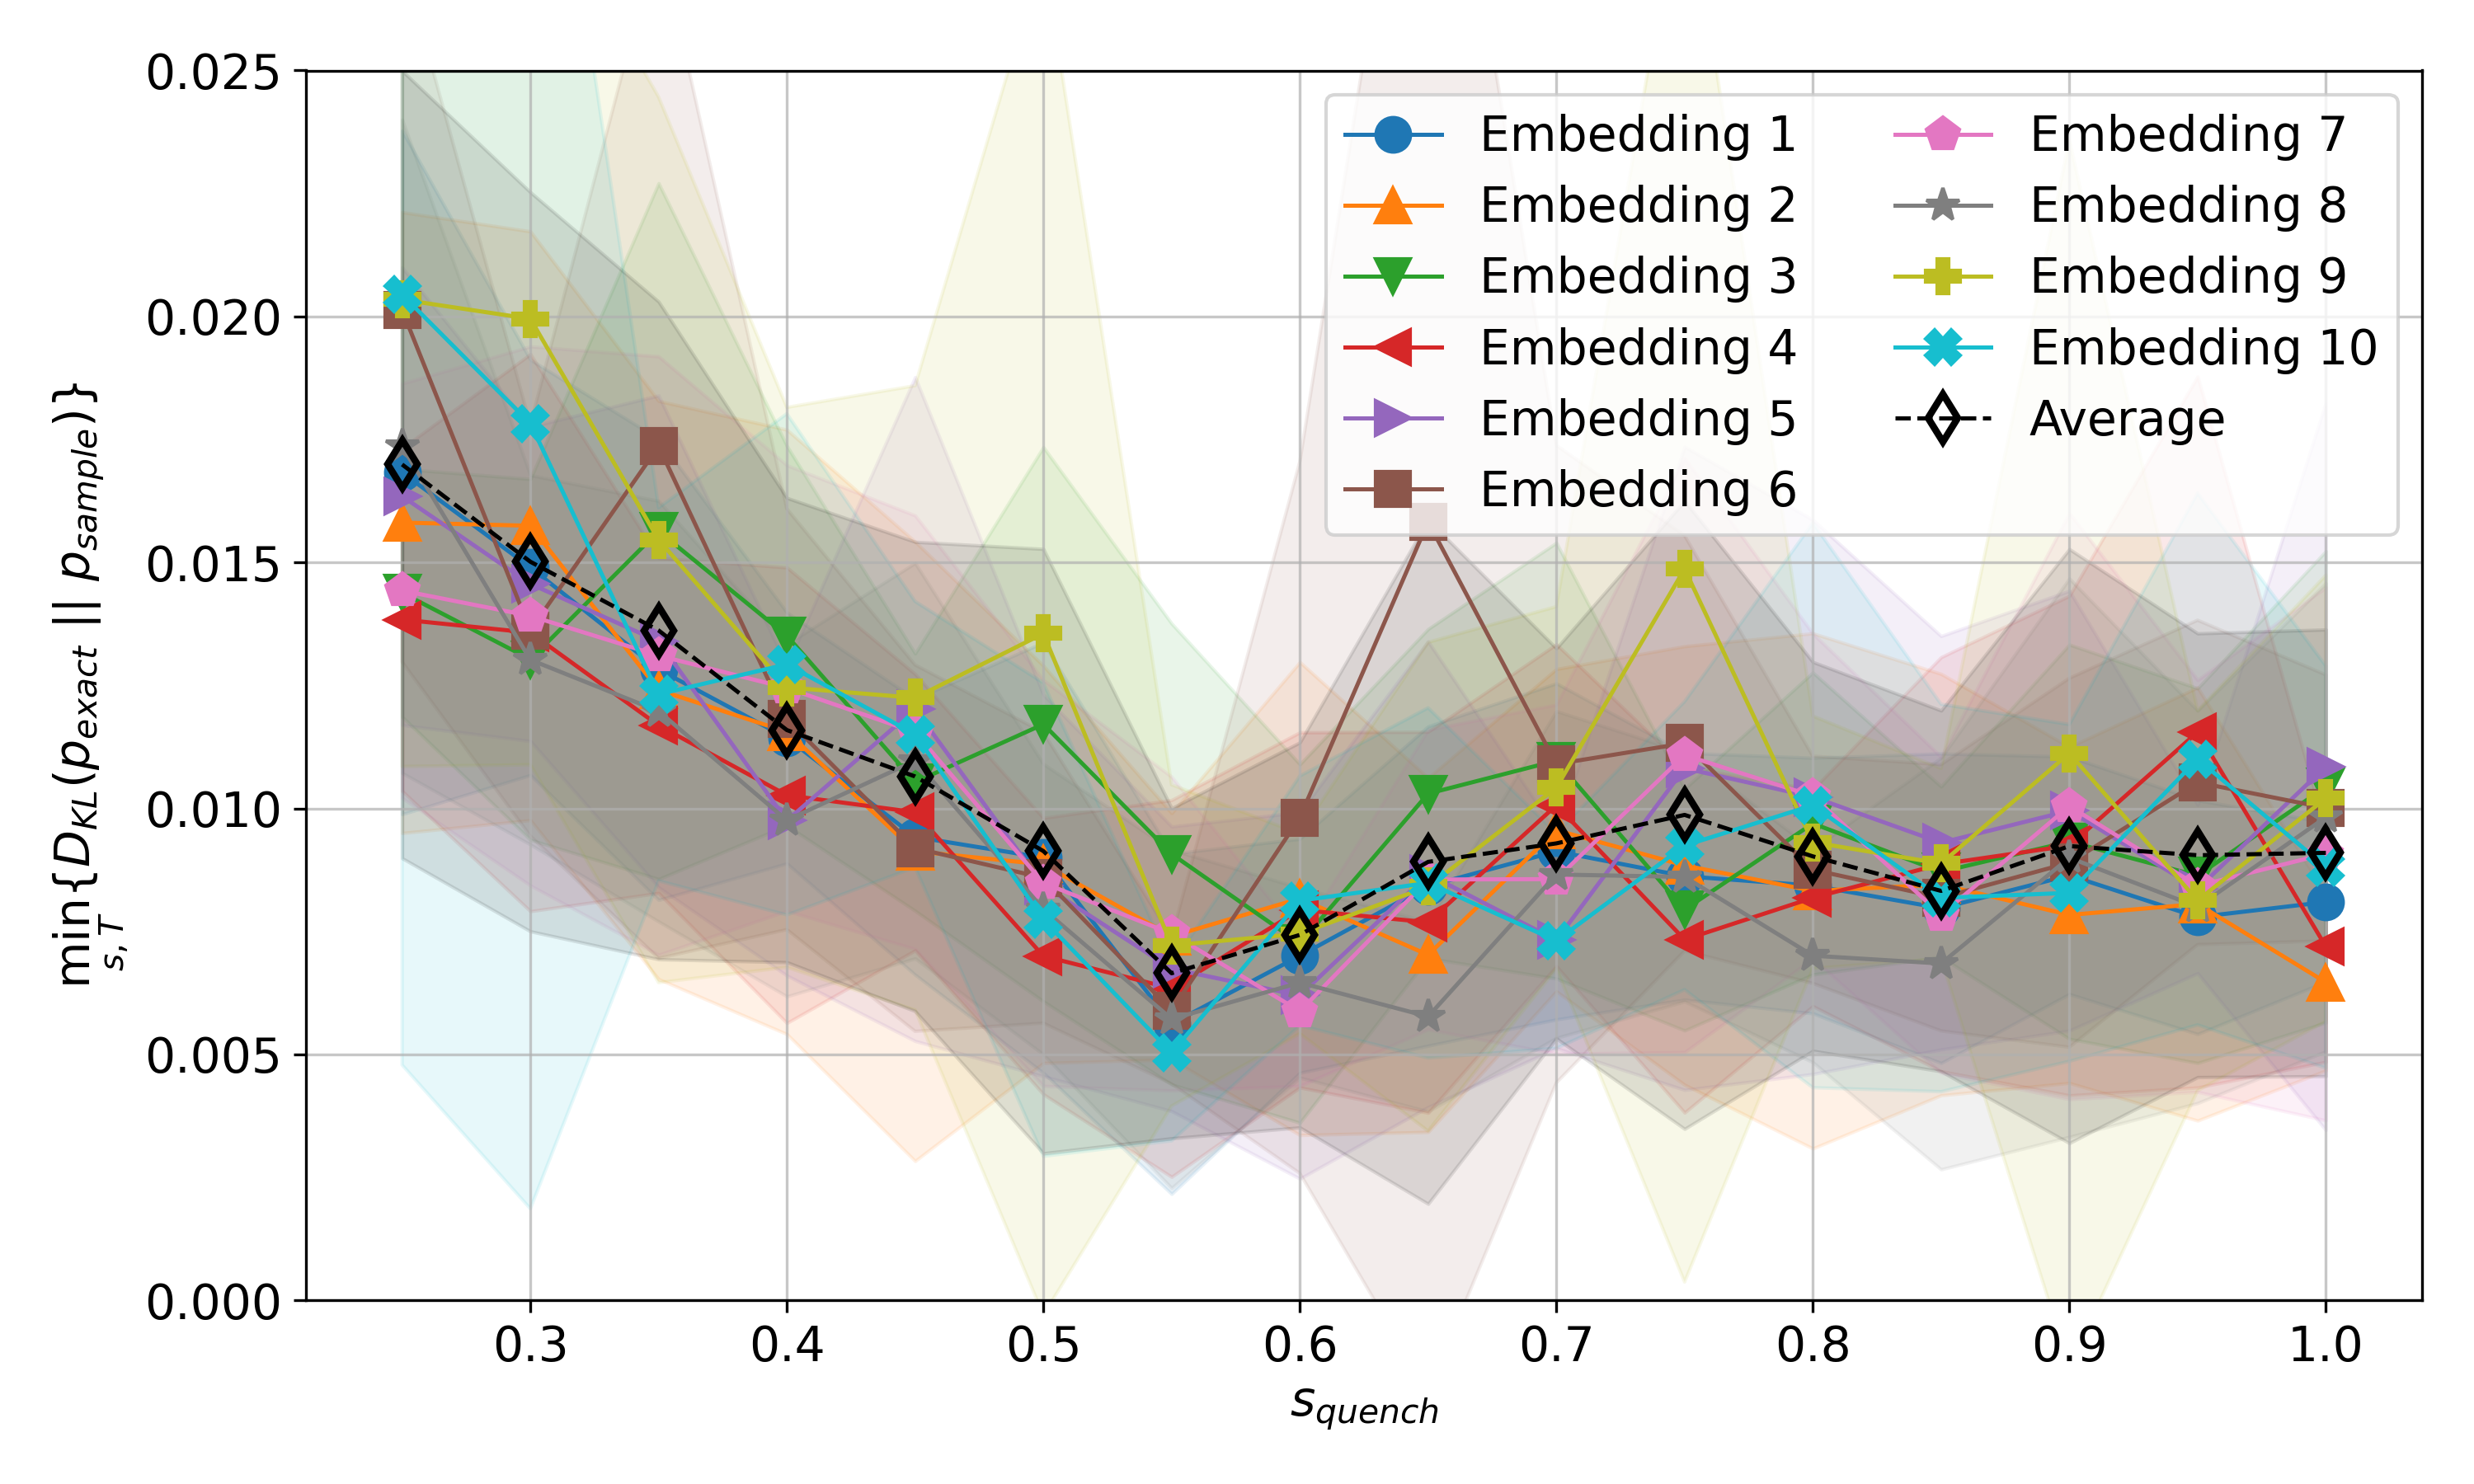
\includegraphics[width=1\linewidth]{8x4/exact_analysis/01/embedding_01/kl_divergence_mins.png}
    \end{figure}
\end{frame}
\begin{frame}
    \frametitle{\( h_i, J_{ij} \sim \mathcal{N}(0, 0.01) \)}
    \begin{figure}
        \includegraphics[width=0.85\linewidth]{01/plots/heatmaps/embedding_01/t_pause=10.0,s_pause=0.5,pause_duration=0.0,quench_slope=2.0.png}
    \end{figure}
\end{frame}

\begin{frame}
    \frametitle{\( h_i, J_{ij} \sim \mathcal{N}(0, 0.1) \)}
    \begin{figure}
        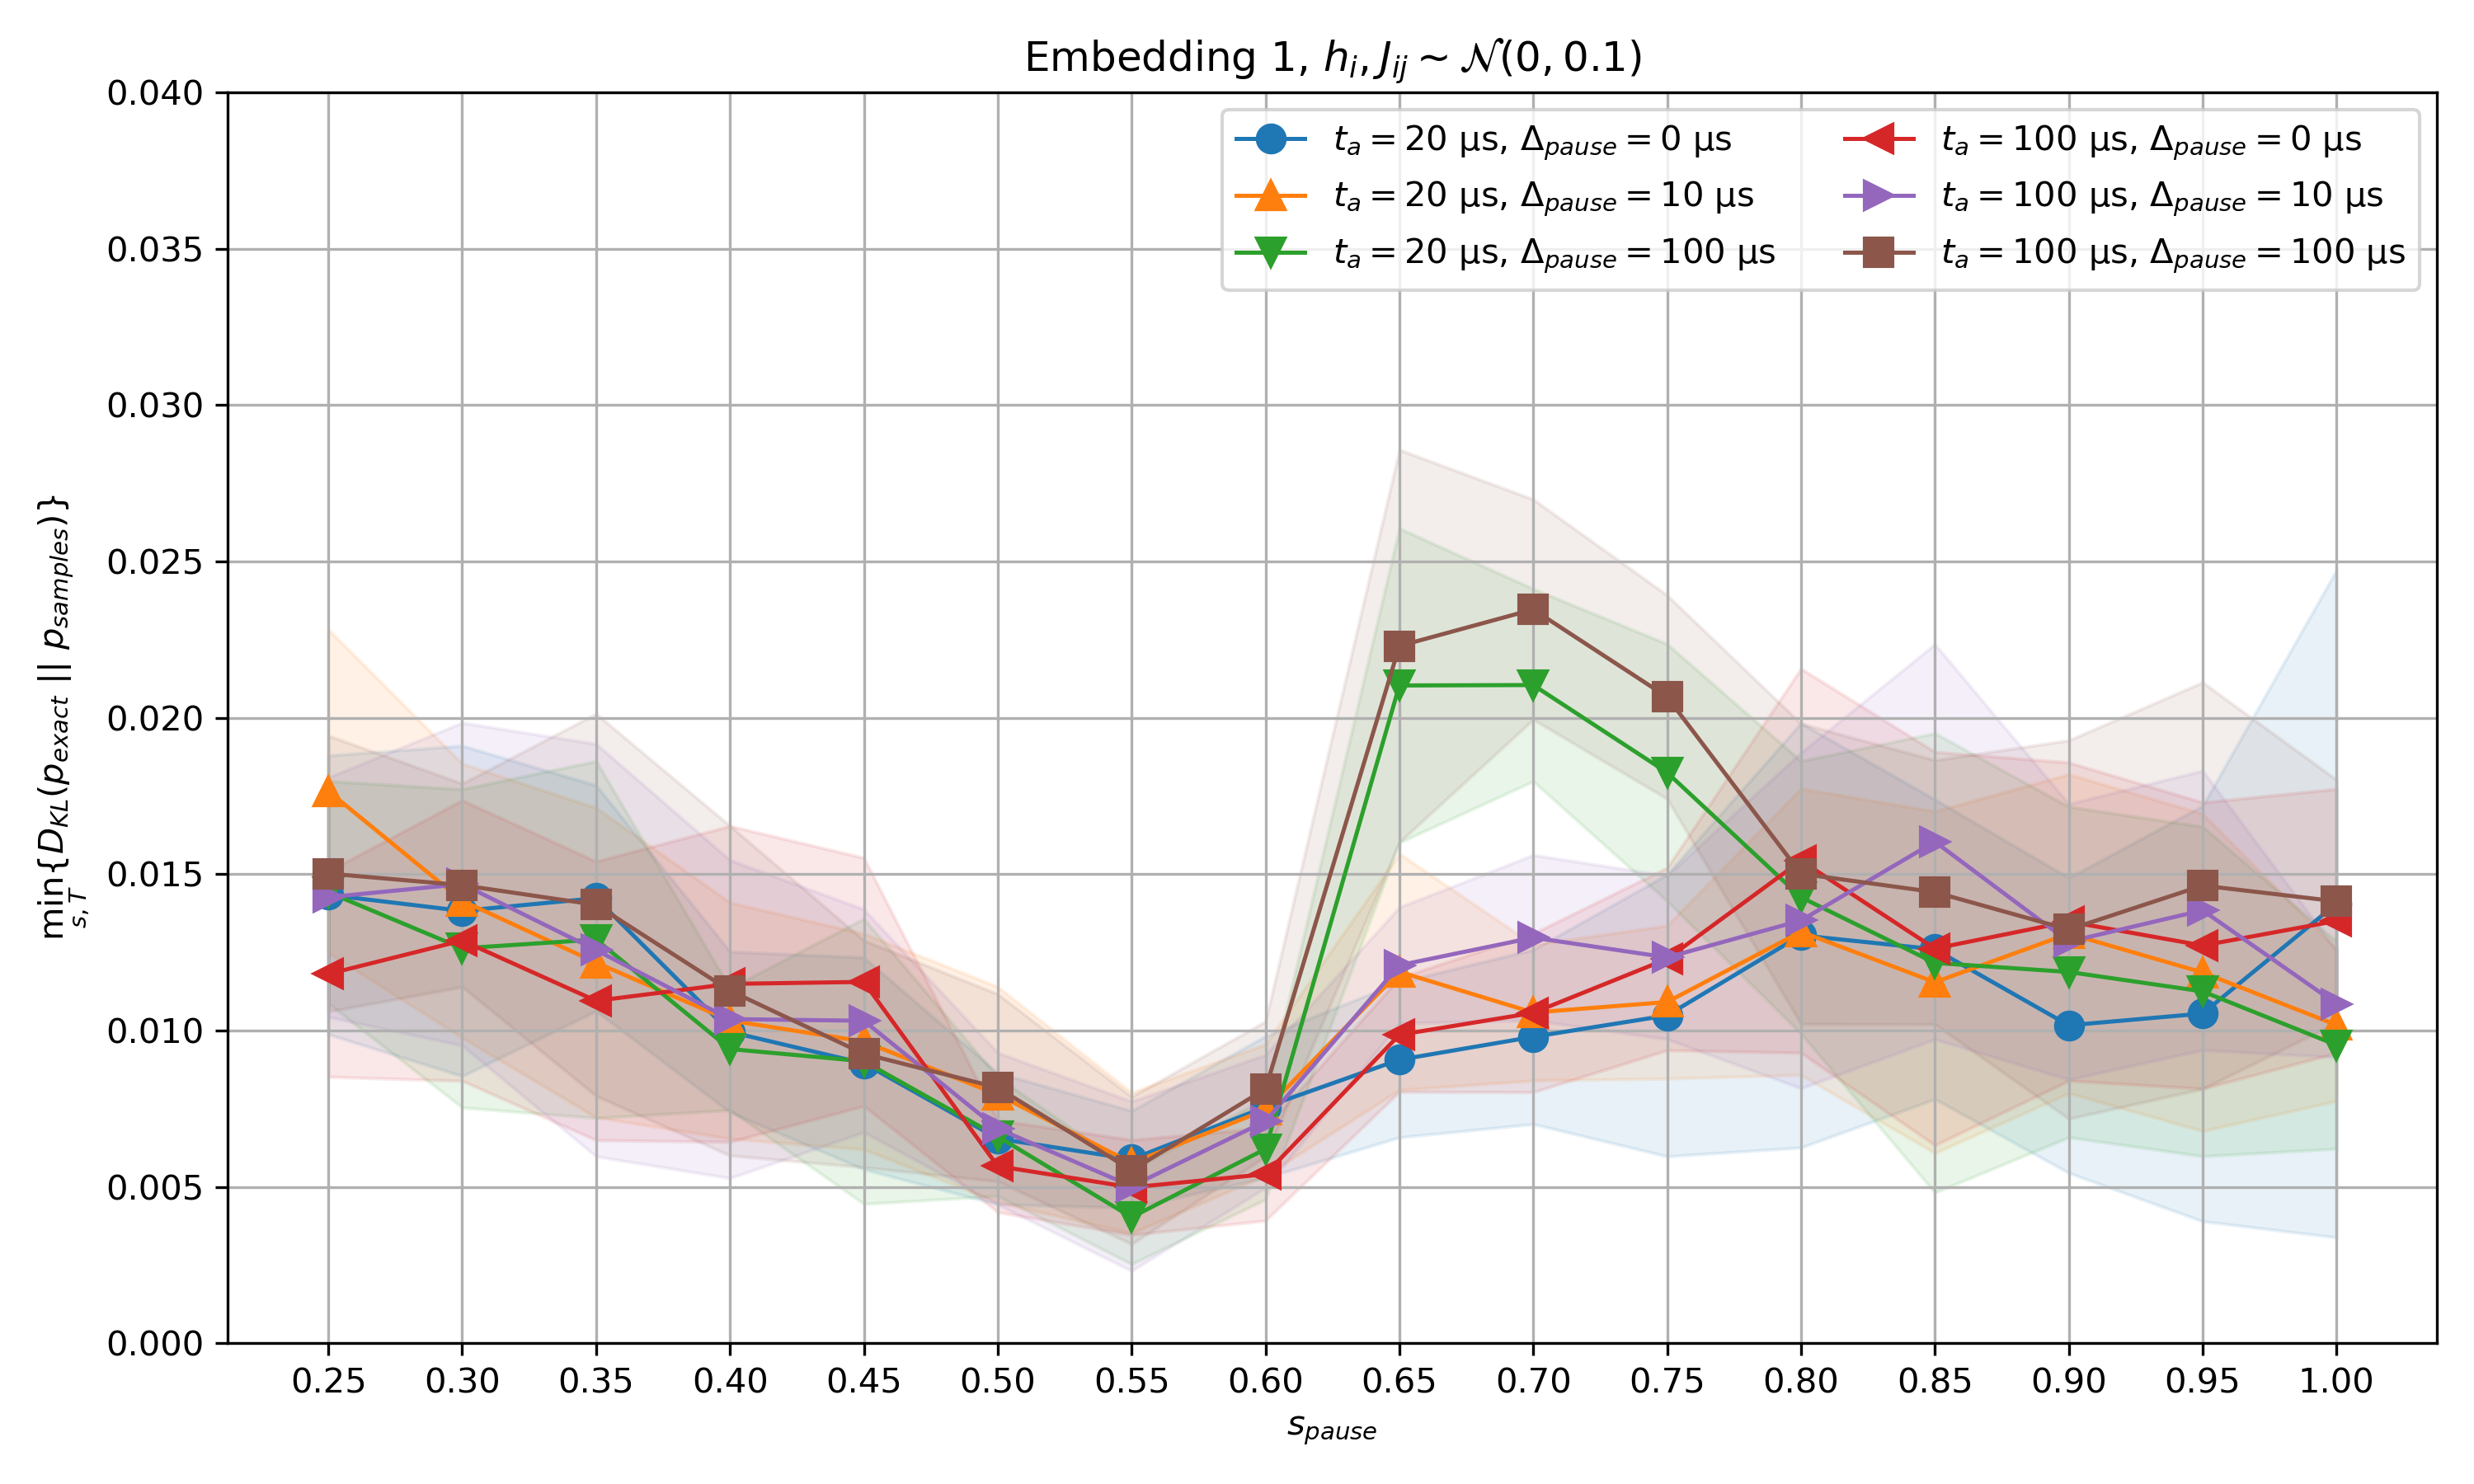
\includegraphics[width=1\linewidth]{8x4/exact_analysis/02/embedding_01/kl_divergence_mins.png}
    \end{figure}
\end{frame}
\begin{frame}
    \frametitle{\( h_i, J_{ij} \sim \mathcal{N}(0, 0.1) \)}
    \begin{figure}
        \includegraphics[width=0.85\linewidth]{02/plots/heatmaps/embedding_01/t_pause=10.0,s_pause=0.5,pause_duration=0.0,quench_slope=2.0.png}
    \end{figure}
\end{frame}

\begin{frame}
    \frametitle{\( h_i, J_{ij} \sim \mathcal{N}(0, 1) \)}
    \begin{figure}
        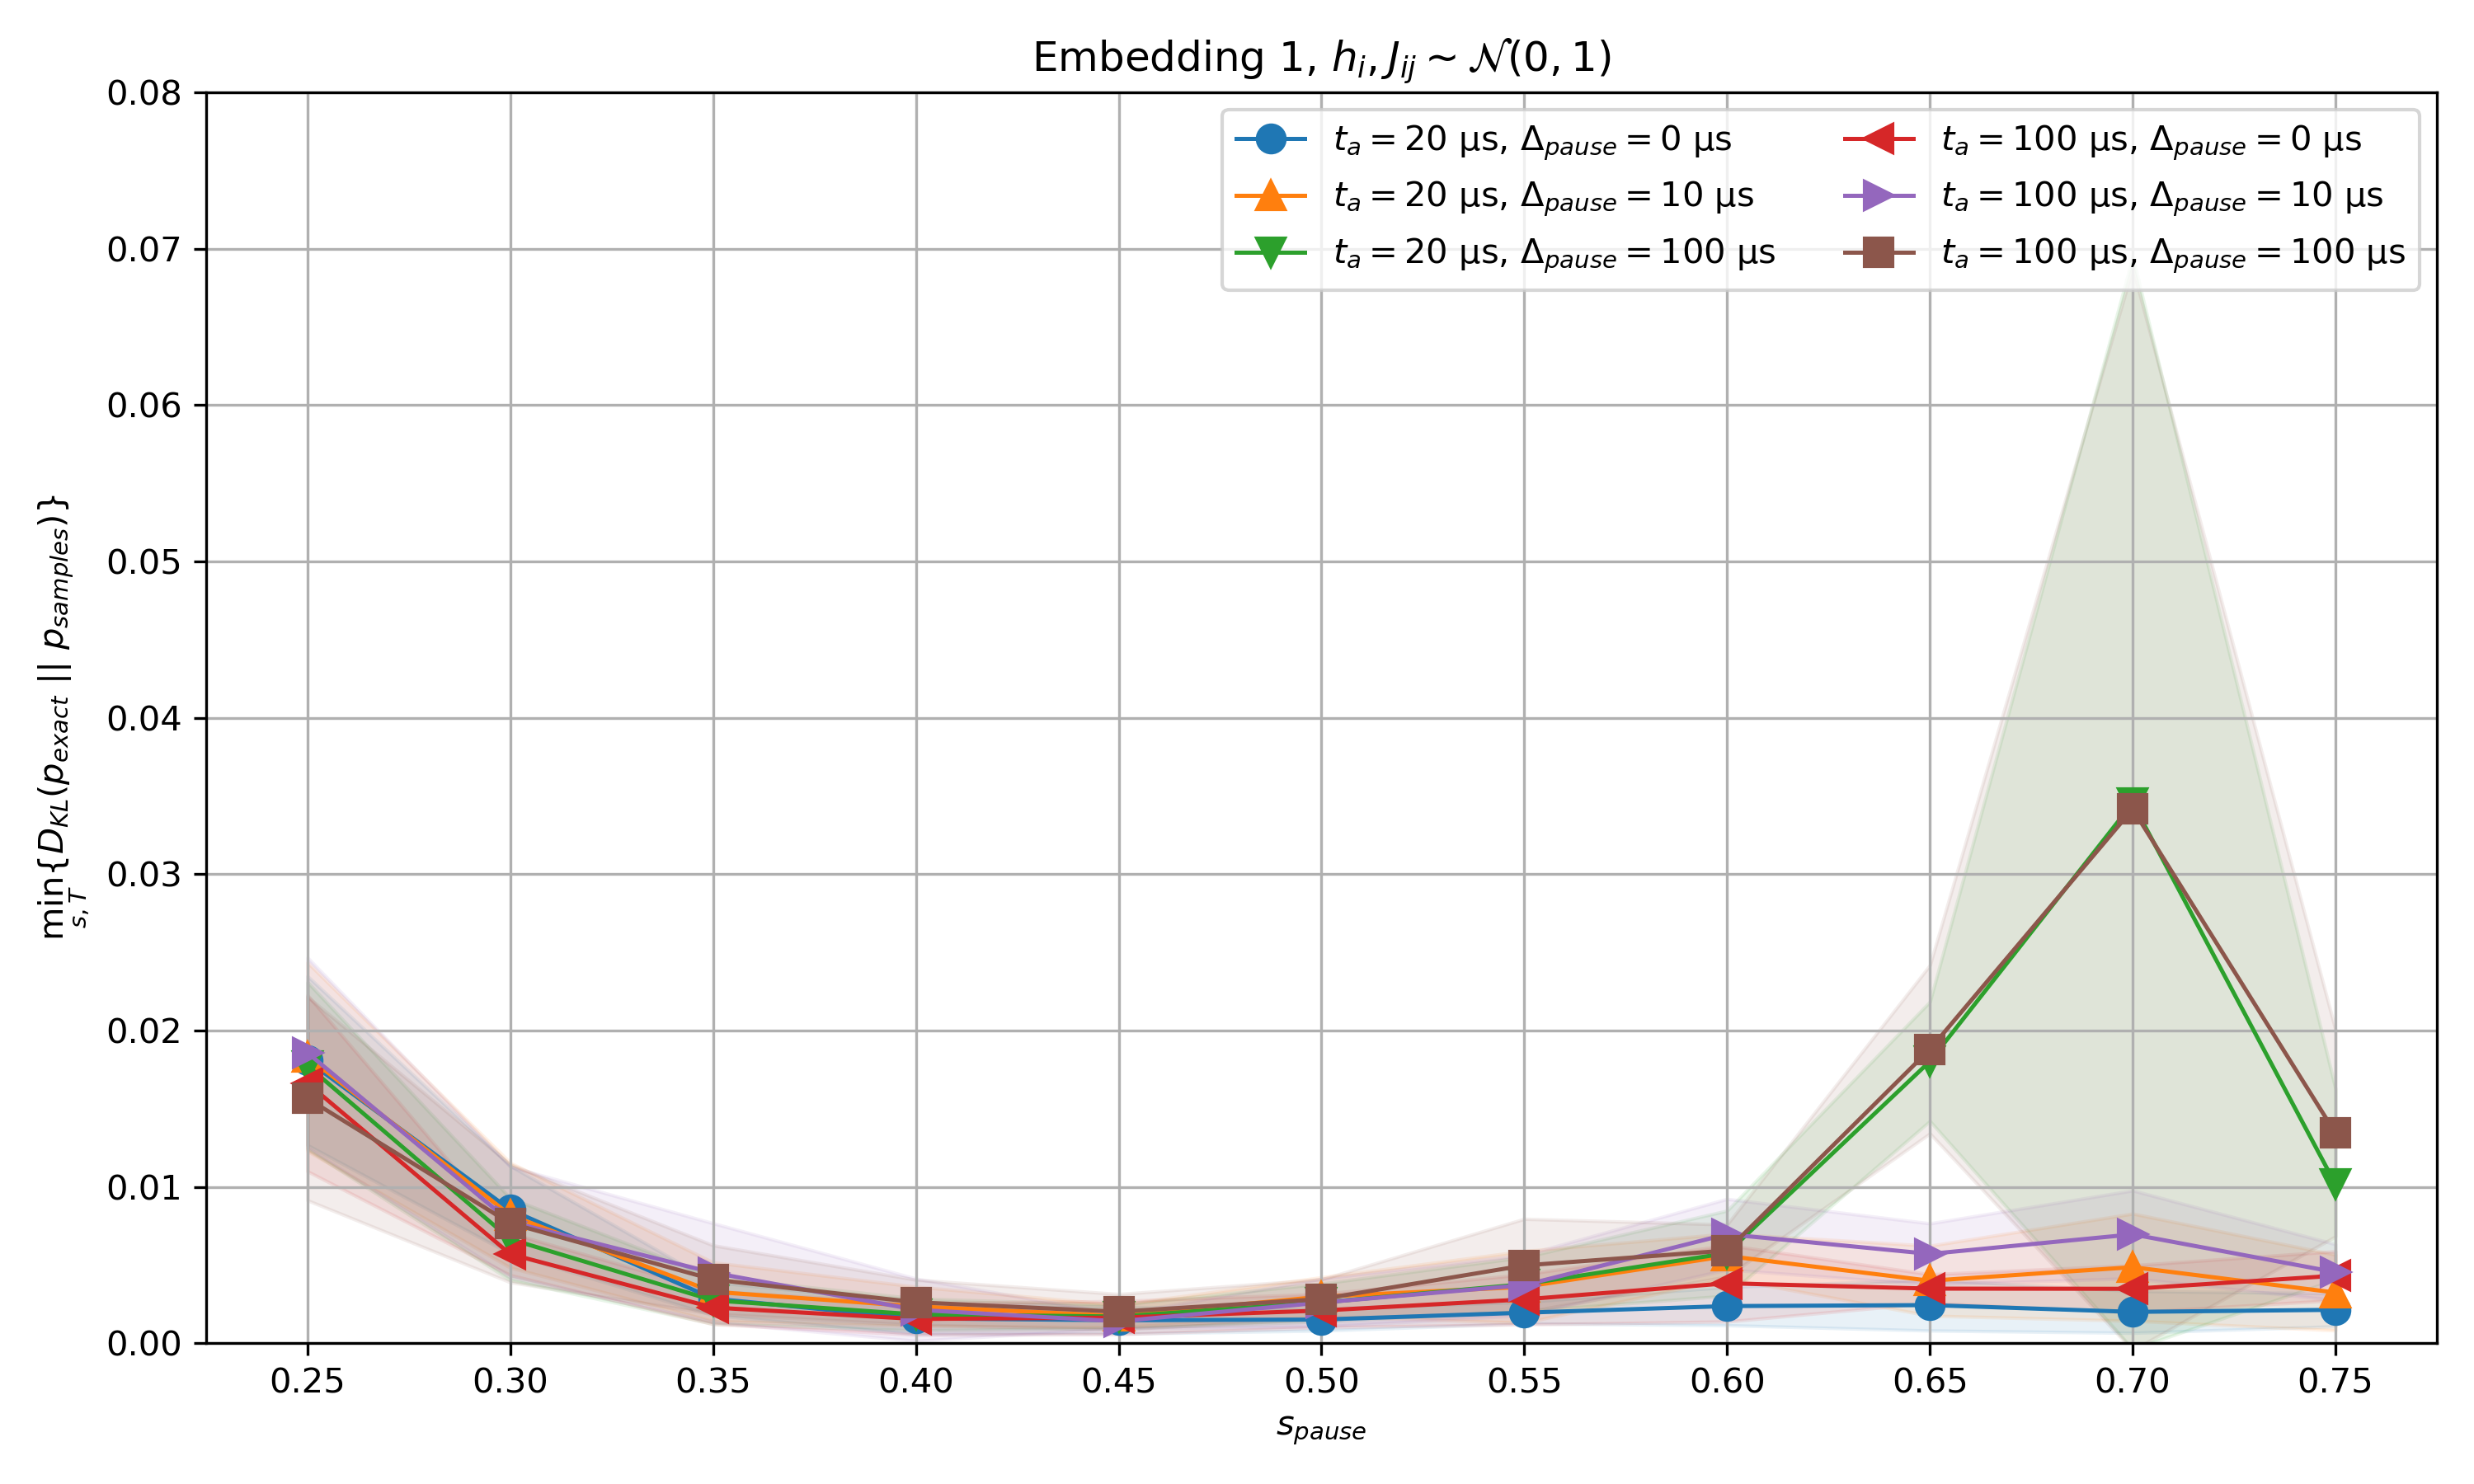
\includegraphics[width=1\linewidth]{8x4/exact_analysis/03/embedding_01/kl_divergence_mins.png}
    \end{figure}
\end{frame}
\begin{frame}
    \frametitle{\( h_i, J_{ij} \sim \mathcal{N}(0, 1) \)}
    \begin{figure}
        \includegraphics[width=0.85\linewidth]{03/plots/heatmaps/embedding_01/t_pause=10.0,s_pause=0.5,pause_duration=0.0,quench_slope=2.0.png}
    \end{figure}
\end{frame}

%----------------------------------------------------------------------------------------
% Exact QBM Tests
%----------------------------------------------------------------------------------------

\section{Exact QBM Tests}
\begin{frame}
    \frametitle{Exact BQRBM Training}
    To verify that the BQRBM works properly, we train a network with 8 visible and 4 hidden units to use as an autoencoder to generate samples from a specified nontrivial distribution at \( s^* = 1.0 \).
    We train the model on 1500 samples from the Gaussian mixture distribution
    \[
        p(x) = \frac{2}{3} \mathcal{N}(x \ | \ -2, 1) + \frac{1}{3} \mathcal{N}(x \ | \ 3, 1)
    \]
    The model allows for the effective inverse temperature to be learned with iterative updates of the form
    \[
        \Delta\beta = \eta (\overline{\braket{E}_\vec{v}} - \braket{E})
    \]
    We set the exact sampler to use an inverse temperature value of \( \beta_{\text{effective}} = 0.5 \) with an initial \( \beta \) to verify that the \( \beta \) parameter can be learned.
\end{frame}

\begin{frame}
    \frametitle{Decreasing KL Divergence}
    \begin{figure}
        \includegraphics[width=1\linewidth]{8x4/dkl_exact.png}
    \end{figure}
\end{frame}
\begin{frame}
    \frametitle{Learning \( \beta \)}
    \begin{figure}
        \includegraphics[width=1\linewidth]{8x4/beta_exact.png}
    \end{figure}
\end{frame}
\begin{frame}
    \frametitle{Learning an Arbitrary Distribution}
    \begin{figure}
        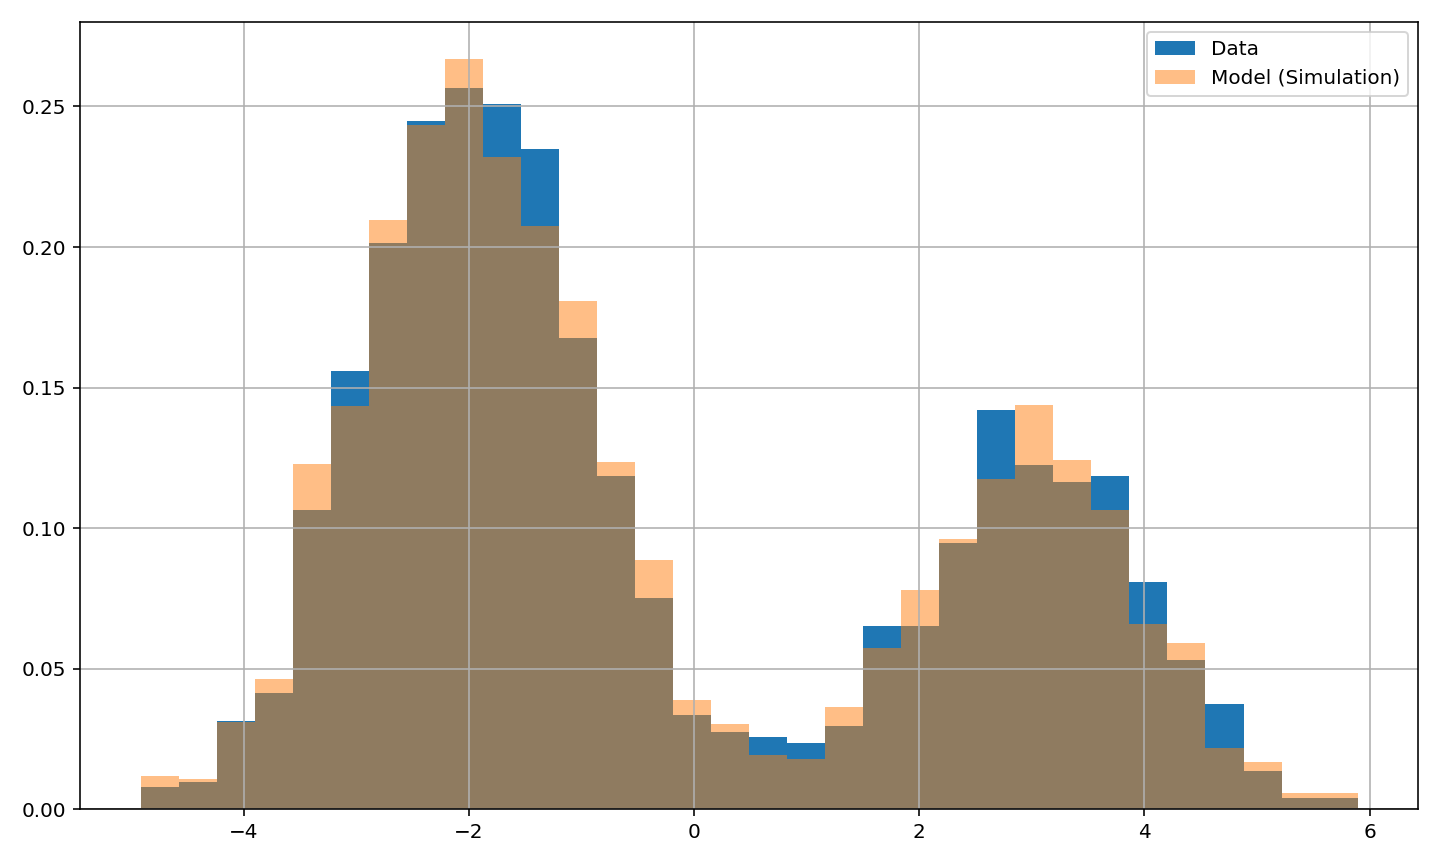
\includegraphics[width=1\linewidth]{8x4/hist_comparison_exact.png}
    \end{figure}
\end{frame}

\begin{frame}
    \frametitle{Decreasing KL Divergence}
    \begin{figure}
        \includegraphics[width=1\linewidth]{8x4/dkl_exact_annealer_comparison.png}
    \end{figure}
\end{frame}
\begin{frame}
    \frametitle{Learning \( \beta \)}
    \begin{figure}
        \includegraphics[width=1\linewidth]{8x4/beta_annealer.png}
    \end{figure}
\end{frame}
\begin{frame}
    \frametitle{Learning T}
    \begin{figure}
        \includegraphics[width=1\linewidth]{8x4/temperature_annealer.png}
    \end{figure}
\end{frame}
\begin{frame}
    \frametitle{Learning an Arbitrary Distribution}
    \begin{figure}
        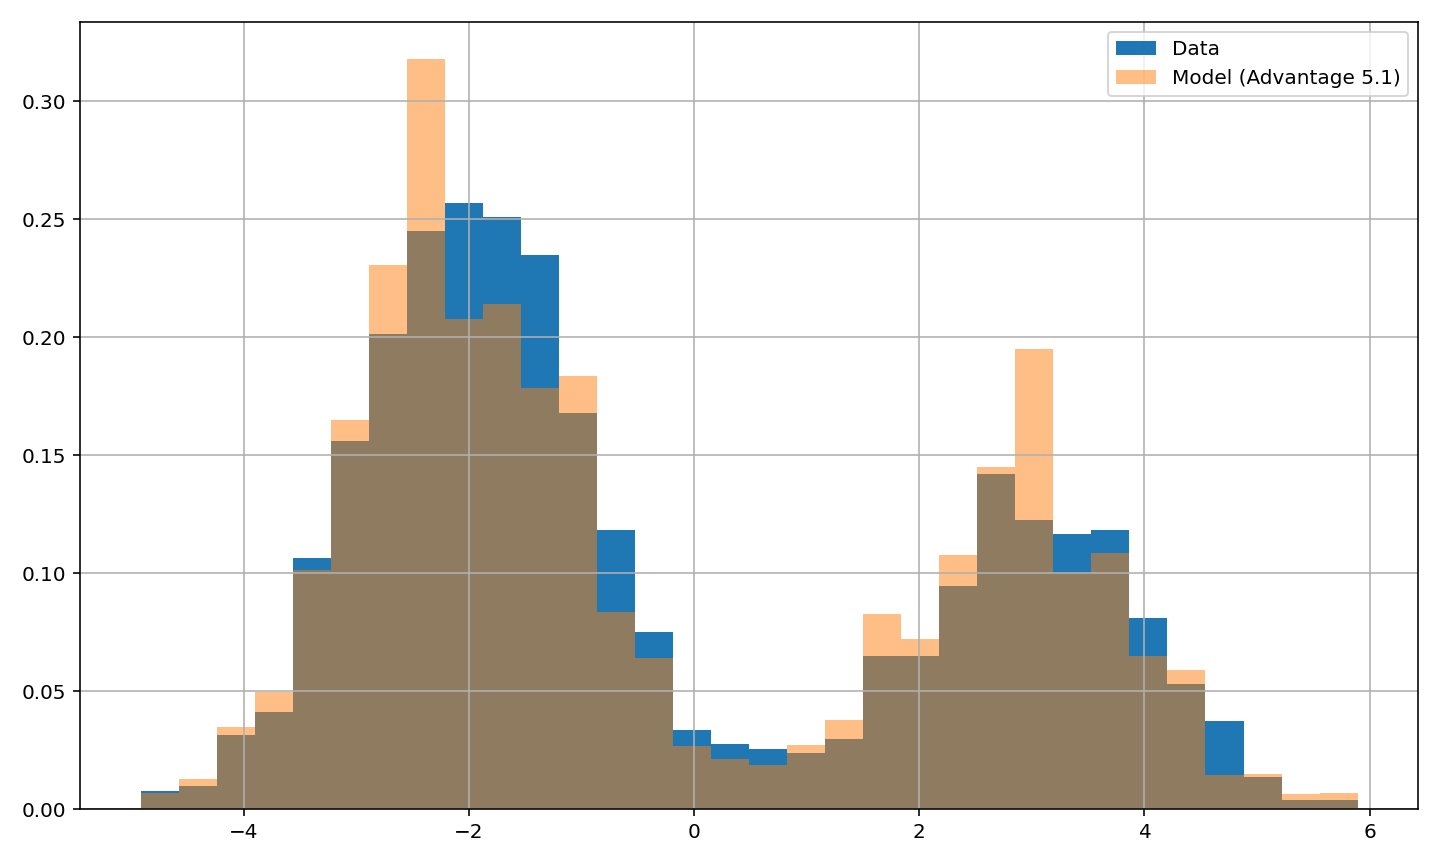
\includegraphics[width=1\linewidth]{8x4/hist_comparison_annealer.png}
    \end{figure}
\end{frame}


%----------------------------------------------------------------------------------------
% References and Resources
%----------------------------------------------------------------------------------------

\section{Next Steps}

\begin{frame}
    \frametitle{To Do}
    \begin{itemize}
        \item Determine a method to choose an embedding and chain strength for the larger model.
    \end{itemize}
\end{frame}

%----------------------------------------------------------------------------------------
% References and Resources
%----------------------------------------------------------------------------------------

\section{References and Resources}

\begin{frame}[allowframebreaks]
    \frametitle{References}
    \footnotesize{
        \bibliographystyle{abbrv}
        \bibliography{../../references.bib}
    }
\end{frame}



\end{document}
